\chapter{Design}
\label{chap:Design}

We aim to design stealthy \ac{SNI} and \ac{ALPN} encryption schemes based
on the basic premise that the 32 octets of the client \var{random}
along with the 32 octets of the \varlegacysessionid{} act as `cover',
which can be replaced with random-looking ciphertext.
There are other fields and extensions to the \ac{CH} message
which could provide additional cover,
but the \var{random} and \varlegacysessionid{}
provide cover of the highest quality; they are always present in a \ac{TLS} 1.3 \ac{CH},
their lengths do not vary between implementations, and they will not
need to be \ac{GREASE}'d.
The designs presented below leverage only these 64 octets of cover in the \ac{CH},
as well as the 32 octets of cover provided by the \ac{SH}\var{.random}.

\section{Discussion of RFC8744 Requirements}

In RFC 8744 \cite{rfc8744-issues} lay out a set of issues and design requirements pertaining to \ac{SNI} encryption, and the aim of this dissertation is design an \ac{SNI} encryption scheme that prioritises the requirement: ``Do Not Stick Out". However, a stealthy \ac{SNI} encryption scheme should of course also fulfill the other requirements listed by \cite{rfc8744-issues} where possible. Here we discuss these requirements and possible approaches to fulfilling them.


We discuss the requirement to "Mitigate Cut-and-Paste Attacks" in more detail in Section~\ref{sec:cut-and-paste-attacks}.

\subsection{Avoid Widely Shared Secrets}

\ac{ECH} avoids widely shared secrets through the use of \ac{PKC},
which is the approach we also adopt for
\ac{SECH} 3.

Our design \ac{SECH} 2
could be deployed with a widely shared secret,
which we recommend against.
As an alternative to sharing the secret
we have designed a bootstrapping mechanism
based on \ac{PSK}s.


\subsection{Enable Multi-Party Security Contexts}
This requirements is about securely allowing the separation of the client-facing server and the backend server. In particular the protocol should protect the client from \ac{MITM} attacks.

We can imagine a naïve design where a client-facing server terminates the \ac{TLS} connection.
This means the client-facing server has to possess the relevant certificate's private key and produce the \ac{CV}.
The servername could be indicated stealthily somehow, e.g. by prefixing it to the application data,
and then the true application data is relayed in the clear (or protected by some other means) to the backend server.
In this design the client never authenticates the backend server, which means the client-facing server can act as a \ac{MITM} and delete, modify, reorder messages to/from the backend server without the client or backend server being able to detect these modifications.


\cite{rfc8744-issues} also point out that backend-server authentication is not sufficient,
and that the client-facing server should also be authenticated.

\ac{ECH} mitigates against \ac{MITM}
by having the client authenticate
the backend server using the regular
\ac{TLS} 1.3 mechanisms,
but additionally there is an implicit authentication that the client-facing server owns the \var{ECHConfig},
i.e. it has the corresponding private key
(In order for the server
to produce the \ac{ECH} \var{accept\-\_confirmation} signal
it has to successfully decrypt the \ac{ECH} payload.).
The cleartext of the payload is hard to 
guess because it contains a 32 octet random,
which makes it hard for an attacker
to fraudulently authenticate as the client-facing server.

\ac{ECH} does not perform encryption of the secret \ac{SNI} parameter in the channel between
the client-facing and backend server,
which means this channel has to be protected
by some other means,
e.g. with a \ac{VPN} or a separate \ac{TLS} connection. The same is true for \ac{SECH}.

\cite{esni} distinguish two modes of operation for \ac{ECH}, shared mode and split-mode.
In shared mode there is a single server which performs the \ac{ECH} decryption {\em and} terminates the \ac{TLS} connection,
whereas in split-mode there is a client-facing server that performs \ac{ECH} decryption and which proxies the remaining \ac{TLS} traffic to and from a backend server which terminates the \ac{TLS} connection.
For \ac{ECH} each server is `aware' of its role in the ongoing connection.
The server can have a different role for different connections,
but within the context of a single connection the server determines its role based on the \var{type} field of the received \var{encrypted\_client\_hello} extension,
if the \var{type} is \var{outer} then the server is the client-facing server,
if it is \var{inner} the server is the backend server.

Figure~\ref{fig:sech-split-mode-accept} shows sequence diagram depicting the flow of messages in split-mode.

\begin{figure}[htb]
\centering
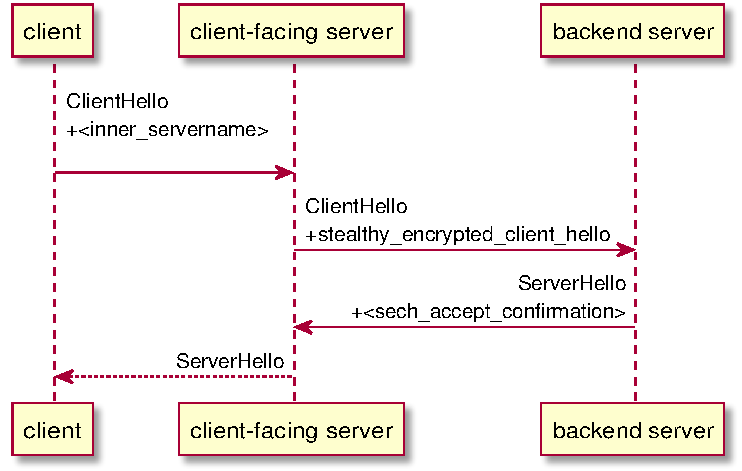
\includegraphics[width=\linewidth]{figure/sech-split-mode-accept.pdf}
\captionsetup{width=.8\linewidth} 
\caption[]{Sequence diagram for a successful \ac{SECH} split-mode handshake. Parameters in angle brackets <> are encoded stealthily in the message.}
\label{fig:sech-split-mode-accept}
\end{figure}

For \ac{SECH} we don't have the luxury of setting
a cleartext \var{type} field to help the server
distinguish its role.
The approach we'll adopt below is to set the \ac{SNI} extension value in the \ac{CHI} to all 0s
as a signal that the server should act as a backend server.
The true \ac{SNI} is encoded elsewhere in the \ac{CHI}.

The motivations for split-mode are:
1. to distribute workload,
and 2. to enhance privacy for the backend server and the user
(the client-facing server can't see application traffic).

One reason for hesitance in deploying split-mode may be that there's low incentive for large providers.
The provider loses access to application traffic,
which means, for instance, it can't implement a \ac{WAF}.
Secondly the deployment and maintenance
of split-mode is more complex.

Issues around \ac{HRR} hijacking
make it challenging to design \ac{SECH}
while maintain stealth,
because it would require coordination of
two backend servers,
the backend server
corresponding to the outer \ac{SNI},
and the backend server corresponding to the inner \ac{SNI}.
Facilitating split-mode remains an open issue in our design.

\subsection{Prevent SNI-based DoS}
\cite{rfc8744-issues} note that in a split-mode deployment the client-facing server
may have more limited resources,
and so may be a target for \ac{SNI}-based \ac{DoS} attacks.
In shared-mode the argument is less relevant.

Our designs of \ac{SECH} 2 and \ac{SECH} 3
facilitate multiple \ac{SECH} keys
via trial decryption.
Increasing the number of keys increases
the cost of processing every \ac{CH} proportionally (whether or not the \ac{CH} is using \ac{SECH}).
In this sense our designs have failed to
fulfill the requirement to prevent
\ac{SNI}-based \ac{DoS}.
But, this can be mitigated by keeping
the number of enabled keys very small.

\subsection{Maintain Forward Secrecy}
Forward secrecy means that if the private key of one of the parties is compromised, then this
does not necessarily mean that
keys used in previous sessions are also compromised.
This is achieved in \ac{TLS} using {\em ephemeral} \ac{DH}.
The \ac{ECH} draft does not provide
forward secrecy of servername encryption because the long term private \ac{KEM} key is static.
The difficulty in providing forward secrecy
for \ac{ECH} is that the
servername ciphertext is sent in
the first flight of messages,
which makes it impossible to
negotiate ephemeral keys.

For \ac{SECH} 3 the case is the same,
but by using the \ac{PSK} bootstrapping
mechanism for \ac{SECH} 2 we achieve
forward secrecy.
This is possible because the \ac{PSK}
bootstrapping mechanism entails an additional previous handshake in which
an ephemeral key can be established.

\section{SECH Specifications}
Here we provide specifications for \ac{SECH} 2 (symmetric encryption only) and \ac{SECH} 3 (\ac{HPKE}-based encryption).
In a later section (\ref{sec:sech1}) we discuss \ac{SECH} 1, a design involving no secrets,
but we did not pursue a thorough design of \ac{SECH} 1 in this work.

\section{SECH 1: Secretless Stealthy Encoding}
\subsection{Motivations and Deployment Scenarios}

There are potential use-cases
for an \ac{SECH} variant
that uses no encryption (and thus
needs no secret)
but such a variant should more properly be called just `stealthy SNI' or `stealthy CH'.

An advantage of such a variant is the very low coordination/infrastructure requirements to get this working.
Client and server simply need to run the same
protocol, with no need for out-of-band secret sharing,
or public key distribution.

Our design for \ac{SECH} 1 does {\em not} offer confidentiality of the \ac{SNI} or \ac{ALPN}.
The aim here is purely to circumvent censorship
in the case of a naïve censor.

As a censorship circumvention method this can be easily detected and prevented, but this it is still possibly useful transiently and at a small scale.
If only a small number of Internet users are using the scheme
then it might successfully evade censorship for a time,
before the censor invests the resources to block it.

This approach could be one element in a strategy of circumvention in depth: using lots of different circumvention methods (including this insecure one) in order to increase the cost of censorship for the censor.

\subsection{Design}
It turns out that \ac{SECH} 1 can be implemented 
by running \ac{SECH} 2 (which we'll describe below),
except using a publicly known \varsechlongtermkey{}.

The basic idea is to use a symmetric key encryption to encrypt the
inner \ac{SNI} and \ac{ALPN}, and then replace the \var{random}
and \varlegacysessionid{} fields of the \var{ClientHello}
with the ciphertext. Since the ciphertext is pseudorandom
a censor is forced to perform a decryption operation using
the publicly known key in order to detect \ac{SECH} 1.

Some of the design choices we lay out for \ac{SECH} 2 are overkill
for \ac{SECH} 1.
For instance the acceptance confirmation signal
could be dropped in the case of \ac{SECH} 1.
Due to the limited use-cases for \ac{SECH} 1, however,
we have decided to focus our efforts on designing a secure
\ac{SECH} 2, and neglect to expound here a
version of \ac{SECH} 1 optimised to its particular
design motivations and requirements.

\subsection{Implementation Notes}
The implementation of \ac{SECH} 2 can be used to run \ac{SECH} 1
by configuring the \varsechlongtermkey{} with a publicly
known value such as the 32 byte null string.
\section{SECH 2: Static Secret Shared OOB}
\subsection{Motivations and Deployment Scenarios}

The amount of `cover' available in the TLS 1.3 \ac{CH} message in which we can hide information without differentiating the message from an a normal TLS 1.3 message is limited.
By using only a symmetric encryption algorithm as the basis for sending the stealthy information there is a smaller overhead than for \ac{HPKE}.

While more cover is potentially available we
pursue a design here that leverages only the
\var{random} and \var{legacy\_session\_id} fields,
as explained in Section~\ref{sec:sech-cover-constraints}.

% Other fields/extensions with values that {\em may} look random (and thus might provide cover) are the cipher suite GREASE values, the PSK identity, the \var{key\_share} itself.
% However, the cover provided by these fields/extensions would be less certain because they differ across situations/implementations of TLS. Using these effectively as cover for stealthy bits would involve mimicking the behaviour of a specific implementation in order not to stick out.


% [ ] if the client and server can share the OOB secret securely then we can implement a highly stealthy and cryptographically secure inner SNI
The \ac{AEAD}-only encryption we'll use here
sticks out less than asymmetric encryption.
Asymmetric ciphertexts contain more structure
than symmetric ciphertexts.
With an asymmetric cryptosystem there is
a mathematical relationship between the ciphertext and the private key,
which results in the bytes of the ciphertext being non-uniformly distributed.

% [ ] since the server does not have to publish a public key (as in ECH), it is possible to hide the fact that the server is support SECH from all except the client who knows the OOB secret

% [ ] the secret could be shared amongst multiple clients, allowing for some scale of deployment, but this protocol is certainly not appropriate for internet scale deployments (millions of clients). The more widely the secret is shared the more likely it is to be leaked.
A major challenge with the \ac{AEAD}-only approach
is scaling to multiple users. We could scale by sharing the \varsechlongtermkey{} to
multiple users, but this violates the requirement to `avoid widely shared secrets'.
Another approach would be to enable a distince \varsechlongtermkey{} for each client-server pair,
but this entails costly trial decryption.
Our preferred approach involves using the \ac{PSK} system to bootstrap a shared secret between the client and client-facing server,
which can be used as the \varsechlongtermkey{}
in a subsequent connection.

This design is {\em not} forward secret in the case of repeated use of the \varsechlongtermkey{}.
However, by repeatedly using the \ac{PSK} bootstrap step we can achieve forward secrecy for the inner servername.

\subsection{Design}

We assume the client and client-facing server have some way to securely share a secret out-of-band; call this secret $s$ or \varsechlongtermkey{}.
The shared secret should be a random string of at least 32 octets, or a longer string with at least that much entropy.

The client wishes to communicate \var{sech\_inner\_servername} and \var{sech\_inner\_alpn} secretly and stealthily to the client-facing server.
The maximum length of the \ac{SECH} payload is \sechtwoservernamelen{}.
The \var{sech\_inner\_servername} is concatenade with \var{sech\_inner\_alpn} (separated by the null byte)
and this is padded
with a suffix of zeros to yield \var{sech\_payload} which is \sechtwoservernamelen{} octets long.
The \var{sech\_inner\_alpn} is optional and may have 0 length.
The client also generates a session-specific \sechtwoivlen{} octet \nonce.
The plain text for encryption $pt$ is the \sechtwoservernamelen{} octet \var{sech\_payload} concatenated with a \sechtworandomlen{} byte inner random.

The session \ac{SECH} 2 encryption key $sk_c$=\var{sech\_session\_secret} is computed as defined in Listing~\ref{lst:sech2-derive-secret}.

The client should ensure that it has never used the $(\nonce,sk_c)$ pair before, but ensuring that $(\nonce,sk_c)$ are never reused globally may not be feasible.
The $(\nonce,sk_c)$ should never be used twice by any clients,
but if there a multiple clients that do not coordinate this will be impossible to guarantee.
However, the fact that $sk_c$ is both secret and fresh
makes it difficult for a attacker to exploit \nonce brittleness. % TODO: move to evaluation

We note that the \var{random} and \varlegacysessionid{} give us 64 octets in which we hide the \ac{SECH} 2 offer, and we call this cover field $c$.
This cover is occupied as depicted in Figure~\ref{fig:sech2-cover}.

To construct \ac{CHO} the client first construct the \ac{CH} as specified RFC 8446,
but stops before computing the \ac{PSK} \var{binders}.
Also bytes \sechtwocipheroffset{} to 64 of $c$ need not be randomly generated,
and bytes 0 to \sechtwocipheroffset{} are replaced with the \ac{AEAD} \nonce.

The \ac{AEAD} encrypted text has length \sechtwocipherlen{} and is placed in bytes \sechtwocipheroffset{}  to \sechtwocipherend{} of $c$, as depicted in Figure~\ref{fig:sech2-cover}.

% At last the \ac{PSK} \var{binders} are computed, if necessary, yielding the \ac{CHO}.

We define \var{ClientHelloOuterAAD} as a clone of \var{ClientHelloOuter}, except with bytes 12 to 64 of the cover $c$ set to 0s, and if the \var{pre\_shared\_key} extension is present then the \var{binders} field is set to all 0s.
The session key $sk_c$ can only be computed after \var{Client\-HelloOuterAAD} is known.
The secure derivation of $sk_c$ depends on the entropy of the \var{key\_share} extension and/or the \ac{PSK} identity included in \var{ClientHelloOuterAAD}.
% [] ] TODO: what if key\_share is not included, e.g. for PSK-only handshake? Reject SECH?

%the transcript of \var{ClientHelloInner} message, which is \var{ClientHelloOuter} but with: 1. the encrypted AEAD output replaced with the plain text \var{sech\_inner\_servername} and \var{sech\_inner\_random}, as well as 2. the \var{extension\_data} field of the \var{server\_name} extension set to all 0s with the same length as the cover value for \var{server\_name} (The backend server does not learn the cover SNI used). The AEAD MAC $t$ is left in \var{ClientHelloInner}.

\begin{listing}[htb]
\centering
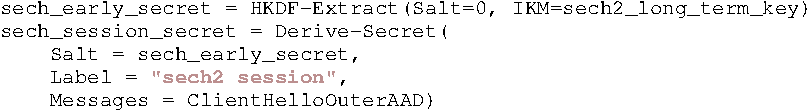
\includegraphics[width=\linewidth]{figure/sech2-derive-secret.pdf}
\captionsetup{width=.8\linewidth} 
\caption[SECH 2 Derive Secret]{Derive $sk_c$, the secret key that will be used by the client to encrypt $pt$ which has the inner \var{CH} data.}
\label{lst:sech2-derive-secret}
\end{listing}

The client encrypts $pt$ (authenticating $aad$) with $(\nonce,sk_c)$ using AES-128-GCM, producing a \sechtwotaglen{} octet authentication tag $t$ and the \sechtwocipherlen{} octet encrypted text $ct$. The \ac{CHO} has $c:=\nonce||ct||t$. The placement of the required values in cover $c$ of the \ac{CHO} is depicted in Figure~\ref{fig:sech2-cover}.
Finally the \ac{PSK} \var{binders} are inserted, which digest the \nonce, $ct$, and $t$.

\begin{figure}[htb]
\centering
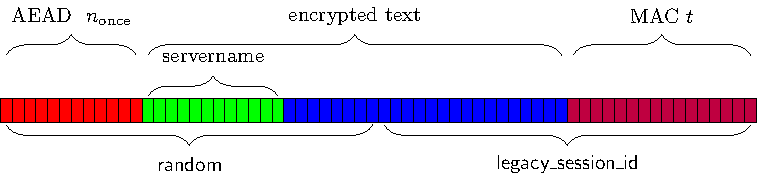
\includegraphics[width=\linewidth]{figure/sech2-cover.pdf}
\captionsetup{width=.8\linewidth} 
\caption[SECH 2 Cover]{Locations of AEAD inputs and outputs in the 64 octets of \ac{CH}\var{.random} and \ac{CH}\var{.legacy\_session\_id}. The cipher text $ct$ and MAC tag $t$ outputs are a function of $iv$, $sk_c$, $pt$, and $aad$: $(ct,t)=\text{AEAD}(iv,sk_c,pt,aad)$.}
\label{fig:sech2-cover}
\end{figure}

A cooperating server in possession of \varsechlongtermkey{} that receives a \ac{CH}
first constructs \var{ClientHelloOuterAAD}, then $sk_c$,
and attempts to decrypt and authenticate $ct$.
If decryption/authentication are unsuccessful the server continues with the \ac{TLS} 1.3 handshake as normal.
If successful, the client-facing server forwards \ac{CHI} to the backend server identified by the inner server name.
If the inner server name does not identify a backend server then the client-facing server continues the \ac{TLS} 1.3 handshake as if \ac{SECH} 2 is disabled.

The \ac{CHI} message  is a clone of \ac{CHO} but with:
1. the encrypted AEAD output $ct$ replaced with the plain text $pt$, as well as
2. the \var{extension\_data} field of the \var{server\_name} extension set to all 0s with the same length as the cover value for \var{server\_name} (The backend server does not learn the cover \ac{SNI} used).
The \ac{AEAD} \nonce and \ac{MAC} $t$ are left in \var{ClientHelloInner}.

The backend server can distinguish a \ac{CHI}
from a regular \ac{CH} by the \var{server\_name} extension.
If the \var{extension\_data} field of the \var{server\_name} has all 0s it is treated as a \var{ClientHelloInner}.
Otherwise it should be treated as a regular \ac{TLS} 1.3 \ac{CH}.
Note that if an attacker can send \ac{CH} directly to
the backend server,
then the client's reaction to an all zero \ac{SNI} can break
channel-level \ac{PC}.
For this reason the backend server must only process messages
from the client-facing server as \ac{CHI}s.
Authentication of the client-facing server is beyond the scope of this specification.
Also, a server tha receives a \ac{CH} whose \ac{SNI} is all 0s must abort with an appropriate alert. % TODO: how do clients typically react to an all zero \ac{SNI}

The server parses the plaintext $pt$
to retrieve the inner server name and inner \ac{ALPN} list
(if present)
in order to select an identity.
At this point the backend server might respond with \var{HRR} or \var{ServerHello}.
As discussed in Section~\ref{sec:hrr-hijacking} in the case of a \var{HRR}
the client and server essentially abandon the attempt to complete the \ac{SECH}
handshake successfully and craft the remaining messages solely for the purpose
of maintaining stealth.
This means the server should select an identity corresponding to the outer \ac{SNI}.
This can be achieved easily in shared-mode, but not split-mode,
since in split-mode the backend server for the outer \ac{SNI}
will not have seen the \ac{CH} or \ac{HRR} messages
needed for the transcript.
It is for this reason that our design of \ac{SECH} 2 does not work in split-mode.

%If the server accepts the first \ac{CHO}
%\ac{SECH} can proceed.
%Whereas in \ac{ECH} the acceptance signal is always sent in the server's first message
%(whether it is a \var{HRR} or \var{SH}),
%for \ac{SECH} 2 the acceptance signal is always in the \var{SH}.
%The client-facing server forwards these (and subsequent) messages to the client unaltered.
If the backend server accepts the parameters of \ac{CHI}
and accepts the inner servername identified in $pt$,
then it responds with a special \ac{SH} containing an \ac{SECH} acceptance signal.
Also, if using certificate-based authentication, then the later \ac{tlsC} message should contain a certificate identified by $pt$.

\begin{listing}[H]
\centering
\fbox{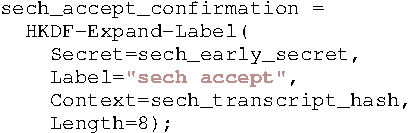
\includegraphics[width=.7\linewidth]{figure/sech2-accept-function.pdf}}
\captionsetup{width=.8\linewidth} 
\caption[SECH 2 Accept Confirmation]{The function used to calculate the SECH 2 acceptance signal using the \var{HKDF-Expand-Label} function defined in Section 7.1 of RFC 8446 (\cite{rfc8446}). The \var{sech\_early\_secret} is derived from $s$ as defined in Listing~\ref{lst:sech2-derive-secret}, and \var{sech\_transcript\_hash} is described in Listing~\ref{lst:sech2-transcript-hash}.}
\label{lst:sech2-accept-function}
\end{listing}

The \ac{SECH} 2 acceptance signal is 24 octets long and placed in the first 24 bytes of the \ac{SH}\var{.random},
such that it does not overlap with the \ac{ECH} acceptance signal.
It is a function of a hash of the transcript of the handshake so far, \varsechtranscripthash{},
and $s=$\varsechlongtermkey{}.
We define \varsechacceptconfirmation{} in Listing~\ref{lst:sech2-accept-function} and \varsechtranscripthash{} in Listing~\ref{lst:sech2-transcript-hash}.

\begin{listing}[H]
\centering
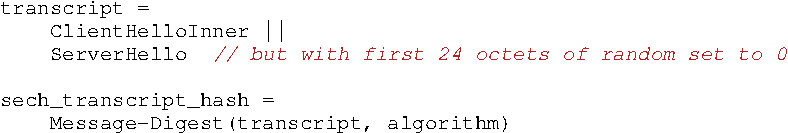
\includegraphics[width=\linewidth]{figure/sech2-transcript-hash.pdf}
\captionsetup{width=.8\linewidth} 
\caption[SECH 2 Transcript Hash]{Specification of the \var{sech\_transcript\_hash} used to calculate \var{sech\_accept\_confirmation}. The \var{algorithm} is the hash algorithm of the negotiated cipher suite for the handshake.}
\label{lst:sech2-transcript-hash}
\end{listing}

% The client uses that secret to encrypt the true target servername as well as a 32 byte secret inner nonce which are hidden in the ClientHello \var{random} and the \var{pre\_shared\_key} extension. The inclusion of the secret inner nonce is necessary to mitigate cut-and-paste attacks.

% More precisely, the client generates a 12 byte initialisation vector for AES-128-GCM. The plaintext is an ASCII encoding of the servername padded with 0x00 up to 12 bytes, appended to the 32 byte inner nonce.
% AEAD is used but the AAD is 0-length. % TODO: might be better to use the transcript hash of ClientHello (with random zeroed) as AAD, (however, if random is zeroed then transcript hash might not change)
% The AEAD tag is truncated to 8 bytes, such that we have a combined 64 bytes to send, which are put into the \var{ClientHello.random} and \var{ClientHello.legacy\_session\_id}. The first 12 bytes contain the IV, the next 12 contain the first 12 bytes of the cipher text, and the last 8 bytes of the \var{random} contain the truncated MAC, and the \var{ClientHello.legacy\_session\_id} is the last 

If the backend server accepts SECH 2 then it makes the SECH inner servername available to the application program via a callback or some other means, which allows the application program to decide whether or not to switch contexts (server certificate etc.).

%\subsubsection{SECH 2 with PSK}
%If a server accepts \ac{SECH} 2 it may issue a ticket referencing a \ac{PSK} that can be used to resume with backend server without stealthy encryption.

%The \ac{PSK} is derived as defined in Listing~\ref{lst:sech2-psk}, which differs from the definition of the PSK defined RFC 8446 in that the label is \var{``sech res''} rather than \var{``resumption''}. This ensures that the standard TLS 1.3 PSK is only used for a connection to the outer servername, whereas the \var{sech2\_psk} is only used for the inner servername.
%\begin{listing}
%\begin{verbatim}
%sech2_psk = HKDF-Expand-Label(
%    resumption_master_secret,
%    "sech res",
%    ticket_nonce,
%    Hash.length)
%\end{verbatim}
%\caption{\label{lst:sech2-psk}Definition of the PSK used when resuming an SECH 2 session.}
%\end{listing}

%Note that this definition of \var{sech2\_psk} is a function of the \var{resumption\_master\_secret}, which is not available to a client-facing server in split-mode.
%Therefore, this type of resumption is not possible in split-mode. % TODO: design PSK resumption for split mode
% TODO: what if sech2_psk and psk are the same, e.g. because they collide when using different ticket_nonces? maybe the label should still be "sech res" but each ticket_nonce should be marked as either sech or non-sech?

\subsection{Distributing SECH 2 access without sharing \var{sech2\-\_long\-\_term\_secret}}

To use a resumption \ac{PSK} (sent via \var{NewSessionTicket}) in TLS 1.3 the PSK
is bound cryptographically to the transcript of the first handshake as well as most of the \var{CH} for the second handshake.
The binding to the first handshake arises because the \ac{PSK} is derived from the key schedule
of the first handshake.
The binding to the second handshake is achieved using the \var{binder} value.
Pseudo-code for the construction of the \var{binder} value is presented in Listing~\ref{lst:binder-pseudocode}.

\begin{listing}
    \begin{verbatim}
early_secret = HKDF-Extract(0, PSK)
binder_key = Derive-Secret(early_secret, "res binder", "")
binder_finished_key = HKDF-Expand-Label(
    binder_key,
    "finished",
    "",
    Hash.length)
binder =
    HMAC(binder_finished_key,
        Transcript-Hash(ClientHello))
    \end{verbatim}
    \captionsetup{width=.8\linewidth} 
    \caption[Pseudo-code for Computation of  \var{binder}]{\label{lst:binder-pseudocode}Pseudo-code of the process used to compute a \var{binder} when using a resumption PSK. The \var{HandshakeContext1} is the transcript of the handshake in which the PSK was derived, and \var{ClientHello} is for a new connection and is truncated so as not to include the \var{binders} list itself. This formulation is tweaked slightly in the case of SECH 2.}
\end{listing}


% [ ] TODO research has anyone done ticket sharing amongst clients before? E.g. client with multiple processes

% [ ] TODO bleichenbacher attack

Sharing the SECH 2 long term secret widely amongst clients would violate the `Avoid Widely Shared Secrets' requirement advocated by \citep{rfc8744-issues}. How do we facilitate connections from large numbers of clients while restricting each long term secret to being shared to only 2 parties? One option is to have a distinct long term secret for each client-server pair. The SECH 2 design specified here can facilitate this through trial decryption, i.e. every \var{ClientHello} processed by the server is checked against each registered secret until one is found to successfully decrypt the inner server name. This approach scales horribly, with the cost of every connection being proportional to the number of registered clients, whether or not those clients are active. But note that this trial decryption process is highly parallelizable.

Our approach to distributing access to the \ac{SECH} 2 capability
exploits \ac{PSK}s, either via gossiping or bootstrapping.
The first step is for a client C1 to establish a resumption \ac{PSK} with
the client-facing server.
For the bootstrap approach: in a subsequent connection the client can use this \ac{PSK}
as if it were the \var{sech2\_long\_term\_key}, while also supplying
the \ac{PSK} identity in the \ac{PSK} extension.
Similarly for the gossiping approach C1 passes the \ac{PSK} (and associated identity)
to another client C2, and C2 uses this \ac{PSK} to perform \ac{SECH} 2.
The backend server will not recognise the \ac{PSK} identity and ignores it.

In split-mode, the initial bootstrap connection is with the client-facing server, whereas
the \ac{SECH} 2 conneciton is with the backend server. This means the second connection
cannot itself be used to establish \ac{PSK}s for subsequent connections.
The bootstrap connection yields some number $n$ of \ac{PSK}s that can be used for connecting
to the backend server, but once these \ac{PSK}s are expended the bootstrap step has to be repeated.

%\begin{listing}
%    \begin{verbatim}
%binder =
%    HMAC(binder_key,
%        Transcript-Hash(ClientHello))
%    \end{verbatim}
%    \captionsetup{width=.8\linewidth} 
%    \caption{\label{lst:binder-sech2-pseudocode-ext}Calculation of \var{binder} for SECH 2 bootstrap \acp{PSK}.}
%\end{listing}

%[ ] The server uses the 32 byte shared secret key as well as the decrypted inner servername to create an 8 byte acceptance signal which is hidden in the ServerHello.random. The 8 byte acceptance signal is computed as \var{sech\_accept\_confirmation = AEAD-encrypt(IV, plaintext="", aad=sech\_inner\_servername, accept\_key).tag}, where IV is the first 12 bytes of the ServerHello.random (uniformly randomly generated), the plaintext is zero-length, the AAD is precisely the inner servername (which does not need to be transmitted because it is known by the client), and \var{accept\_key} is a session-specific key derived using HKDF from the session's master secret and the transcript of ClientHello..ServerHello, but with the last 16 bytes of ServerHello.random set to 0x00. The last 8 bytes of \var{ServerHello.random} are possibly used for an ECH acceptance signal, and the ECH acceptance signal is computed based on the transcript of ClientHello..ServerHello, except with the last 8 bytes of of ServerHello.random set to 0x00. Therefore, if the server is sending an SECH acceptance signal *and* an ECH acceptance signal, the SECH acceptance signal is computed first because the ECH acceptance signal is defined to incorporate the SECH acceptance signal bytes in its transcript hash. To construct the 8 sech\_accept\_confirmation bytes we make use of the HKDF-Expand-Label function defined in RFC 8446 Section 7.1.
    % ```c
    % md = TranscriptHash(ClientHello..ServerHello) // with last 16 bytes of ServerHello.random set to 0x00
    % padded\_sech\_IV = pad(sech\_IV, HashLen)
    % sech\_accept\_confirmation = HKDF-Expand-Label(
    %   HKDF-Extract(padded\_sech\_IV, sech\_symmetric\_key),
    %   "sech ac" || 0x00 || sech\_decrypted\_inner\_servername,
    %   md,
    %   8
    % )
    % ```

\subsection{Design Differences Between SECH 2 and ECH}
[ ] The acceptance signal is always sent in the \var{ServerHello}

[ ] This definition of \var{sech\_accept\_confirmation} is essentially a modification of the ECH \var{accept\_confirmation} defined in Section 7.2 of [TODO cite ECH draft], which we repeat here:
% ```
%   accept\_confirmation = HKDF-Expand-Label(
%     HKDF-Extract(0, ClientHelloInner.random),
%     "ech accept confirmation",
%     transcript\_ech\_conf,
%     8
%   )
% ```

The ECH \var{accept\_confirmation} uses \var{HKDF-Extract(0, ClientHelloInner.random)} as the `Secret' passed to \var{HKDF-Expand-Label}, and \var{HKDF-Extract(0,ClientHelloInner.random)} is confidential (only known to the client and server) because the \var{ClientHelloInner.random} was in the {\em encrypted} \var{ClientHelloInner}. Also, it is essential that \var{accept\_confirmation} can be generated by the backend server in ECH split mode, which is why the salt passed to \var{HKDF-Extract} is the 0 string. While it would be more secure to use a session-specific random value as the salt for \var{HKDF-Extract}, we cannot use the \var{ClientHelloOuter.random} because this value is not available to the backend server (the backend server only processes the ClientHelloInner). The HKDF specification assumes that the salt and IKM passed to HKDF-Extract are indepedent of each other (Section 3.4 RFC 5869), and in particular that the salt values are not `chosen or manipulated by an attacker'.
Since \var{ClientHelloOuter.random} is never processed by the backend server it will not be incorporated into the \var{Finished} message, which means it is not protected from tampering in split-mode. This means an attacker could manipulate \var{ClientHelloOuter.random} and so it should not be used as the salt for \var{HKDF-Extract}.

[ ] In order to facilitate a split mode of operation in a similar fashion to ECH it must be possible for the SECH backend server to produce  the \var{sech\_accept\_confirmation} signal. For the signal described above this entails that the backend server must possess the \var{sech\_symmetric\_key}, meaning \var{sech\_symmetric\_key} would be shared amongst three parties; client, client-facing server, backend server. This violates one of the design requirements listed in Section 3.2 by \cite{rfc8744-issues}; Avoid Widely Shared Secrets.
% \subsection{Security Considerations}

[ ] High probability for situations where an attacker can guess the plaintext, or where there are only a small number of possible plaintexts (SNIs). How does this affect capacity to brute force the secret key? -> Does this mean the SNIs must also remain secret?

\subsection{Implementation Notes}
I have implemented the above \ac{SECH} 2 design in a fork of OpenSSL codebase.
[ ] Error handling
\subsection{Testing}

I have implemented the following basic tests of the \ac{SECH} 2 implementation and \ac{API} using the OpenSSL test infrastructure. Writing tests in this way has the advantage of comfortably allowing granular tests for specific errors and conditions at specific points of execution. A disadvantage is that the tests I have written involving a client and server do not actually use the system's network and hence cannot be easily inspected with external tools like Wireshark.

The \var{test\_sech2\_roundtrip\_accept\_and\_resume\_with\_ticket} first performs the same test as \var{test\_sech2\_roundtrip\_accept} but then additionally tests that the client can reconnect to the server using a resumption \ac{PSK} derived from the first connection. This test revealed an interesting bug and design flaw during development. In an earlier design the \ac{SECH} 2 session key was derived from a transcript of the full \var{ClientHello} including the \var{pre\_shared\_key} extension. However, the \var{binder} values in the \var{pre\_shared\_key} extension are also bound to the rest of \var{ClientHello}. If the session key is bound to the \var{binder} and then used to edit an earlier part of the \var{ClientHello} then the \var{binder} is invalidated. The solution is that the session key should be derived from the \var{ClientHello} up to but not including the \var{binder}, and the \ac{SECH} 2 encryption has to take place before the \var{binder} is calculated.
\section{SECH 5}
\subsection{Motivations and Deployment Scenarios}

[ ] arbitrary access for new clients without coordination from server

\subsection{Design}

A server produces an \var{SECHConfig} which specifies a \ac{HPKE} cipher suite
(\ac{KEM}, \ac{HKDF}, and \ac{AEAD} IDs),
a public key for the \ac{KEM}, and the server
also maintains the corresponding private key for the public key.
For simplicity in this specification we assert that the \ac{HKDF}
and \ac{AEAD} are chosen at \var{SECHConfig}-compilation time.
This is unlike \ac{ECH} where the \ac{HKDF} and \ac{AEAD} are
negotiated for each session.

A client has to securely obtain the \var{SECHConfig} in order to offer \ac{SECH} 5 in a \var{ClientHello}, e.g. using \ac{DoH} or by any other secure and confidential means.

The client first produces the \var{ClientHello} as would be done normally
for \ac{TLS} 1.3 up to the point of computing the \ac{PSK} \var{binder}.

The client instantiates a \ac{HPKE} context using the suite specified in
the \var{SECHConfig} and produces a 32 octet \var{enc}.
As of writing the only \ac{KEM} with a 32 octet \var{enc} in the \ac{IANA} is
the \ac{X25519} \ac{EC}.
The \var{enc} is produced by generating a 32 octet random key, $k$, and then encrypting
that key with the public key from the \var{SECHConfig}.
The \var{random} field is set to value of \var{enc}.

The client concatenates the inner servername and inner \ac{ALPN} list separated by null bytes, and pads this to 16 bytes with 0s. Call the resulting string \var{sech\_cleartext}.
The client creates \var{ClientHelloOuterAAD} which is a clone
of the \var{ClientHello} but with the \var{legacy\-\_session\-\_id} field set to 0s,
and the \var{binders} list truncated off.
Using the \ac{AEAD} specified in the \var{SECHConfig} the client encrypts
\var{sech\_cleartext} with \var{ClientHelloOuterADD} as \ac{AAD}
producing a 32 octet ciphertext \var{sech\_cipher}
(including the 16 byte \ac{AEAD} tag). 
For simplicity we assert in this draft that only \ac{AEAD}s with a 16 byte tag are valid in an \var{SECHConfig}.

% [ ] client encrypts the \var{padded\_servername} with the AEAD specified in SECHConfig, and with key $k$ and a \nonce which is the first 12 octets of the hash of \var{SECH5ClientHelloAAD}, and with \var{SECH5ClientHelloAAD} as AAD, producing \var{sech5\_cipher} which is the concatenation of the encrypted text and the tag $t$

% [ ] \var{SECH5ClientHelloAAD} is the \var{ClientHello} but with the portion in which the AEAD cipher (encrypted text and tag) will be placed set to zero, the size and location of this region depends on \var{SECHConfig}

% [ ] \var{SECH5ClientHelloAAD} is the \var{ClientHelloOuter} but with the \var{random} and \var{legacy\_session\_id} set to all 0s

The client encodes \var{enc} and \var{sech\_cipher} in the \var{ClientHello} \var{random} and \var{legacy\_session\_id} fields producing a partial \var{ClientHelloOuter}
(excluding the \var{binders})
as depicted in Figure~\ref{fig:sech5-cover}.
If the client is using a resumption \ac{PSK} controlled by the backend server
the \var{binders} list is computed
using the synthetic \var{ClientHelloInner} transcript rather
than the transcript of \var{ClientHelloOuter}.

The \var{ClientHelloInner} has the \var{random} field replaced with \varsechinnerrandom{}, and the first 16 bytes of the
\varlegacysessionid{} replaced with \var{sech\_clear}.
Also, the extension data field of the outer \ac{SNI} is set to all 0s.

The client-facing server attempts to decapsulate \var{enc} with the private key associated with \var{SECHConfig} retrieving $k$, on failure 
the client-facing server continues with normal TLS 1.3,
although implementations should ensure that the timing of the response in case of \ac{SECH}
decryption failure is not distinguishable from the case when
\ac{SECH} succeeds.
Using the \ac{HKDF} in \var{SECHConfig} $k$ is transformed into \varsechinnerrandom{}.

% [ ] TODO: Unlike \ac{ECH} we do not support arbitrary numbers \var{SECHConfig}s on the server
% in order to ensure the server response time is consistent and does not reveal \ac{SECH}
% decryption success or failure. 

The client-facing server computes \var{ClientHelloOuterAAD} and the \nonce, and then attempts to decrypt and retrieve \var{sech\_cleartext}, on failure  
the client-facing server continues with a normal TLS 1.3 handshake.

On success the client-facing server constructs \var{ClientHelloInner} by replacing 
the first 16 bytes of \var{ClientHelloOuter}'s \var{legacy\-\_session\-\_id}
with \var{sech\_clear}, and also replacing the \var{random} field
with $k$. Also the \var{extension\_data} of the \var{server\_name} extension is set to all 0s.

The client-facing server forwards \var{ClientHelloInner} to the backend server
(over a channel secured and authenticated by some other means).
The backend server processes this message, detecting the all-zero \ac{SNI} extension value,
and decodes the inner \ac{SNI} and \ac{ALPN} from the \varlegacysessionid{}.

If the backend server needs to negotiate different parameters by sending a
\var{HelloRetryRequest} this message is constructed as in normal \ac{TLS} 1.3.
The \var{HelloRetryRequest} message has no cover for a stealthy acceptance signal.

The subsequent \var{ClientHello2}'s \var{random} and \varlegacysessionid{} fields
must be identical to the first \var{ClientHello} so as not to stick out from normal
\ac{TLS} 1.3. This means the \var{ClientHello2} has no cover for hiding a second
\ac{SECH} payload, which means the \var{ClientHello2} is malleable and 
vulnerable to \var{HelloRetryRequest} hijacking.
Therefore, in the case of a \var{HRR} the remainder of the handshake is simply intended
to prevent revelation to the attacker that \ac{SECH} was attempted, and
the client and backend server give up on the connection.

To achieve this, when a client-facing server receives a \var{ClientHello2} it always
forwards it to the backend server corresponding to the outer \ac{SNI} in the \var{ClientHello2}. Ideally this `cover' backend server should support a superset of
the parameters supported by all \ac{SECH} backend servers such that the \var{ClientHello2}
will be accepted by the `cover' backend.

In the case that no \var{HRR} is triggered the backend server can continue to signal
its acceptance of \ac{SECH}.
The \var{ServerHello} contains a special \var{sech\_accept\_confirmation} value in the last 8 octets of the \var{random} field.


\begin{figure}[htb]
\centering
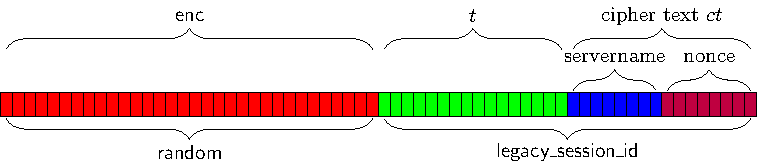
\includegraphics[width=\linewidth]{figure/sech5-cover.pdf}
\captionsetup{width=.8\linewidth} 
\caption[SECH 5 Cover]{}
\label{fig:sech5-cover}
\end{figure}

\subsection{Implementation Notes}